\documentclass[tikz]{standalone}
\usepackage{xcolor}
\usetikzlibrary{3d,calc}


\begin{document}
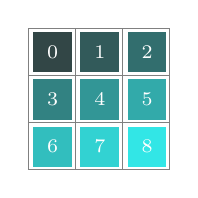
\begin{tikzpicture}[x  = {(1cm,0cm)},
    y  = {(0cm,1cm)},
    z  = {(-.5cm,-.5cm)},
    scale=.6]

  \scriptsize

  \draw [very thin, gray] (0,0) grid (3,3);


  \foreach \pos / \v in {(0,2)/0, (1,2)/1, (2,2)/2, (0,1)/3, (1,1)/4, (2,1)/5, (0,0)/6, (1,0)/7, (2,0)/8} {
      \pgfmathsetmacro{\hue}{70+20*\v} ;
      \draw (0.1,0.05) + \pos node[above right, inner sep=5pt,color=white,fill={rgb,255:red,50;green,\hue;blue,\hue}] {\v} ;
    }

\end{tikzpicture}
\end{document}


